\documentclass[12pt]{article}
%Gumm{\color{blue}i}|065|=)
\usepackage{amsmath, amsfonts, amssymb}
\usepackage[margin=0.5in]{geometry}
\usepackage{xcolor}
\usepackage{graphicx}
\usepackage{amsmath}

\newcommand{\off}[1]{}
\DeclareMathSizes{20}{30}{20}{18}
\usepackage{tikz}


\title{Scratchwork: Galois Theory, Symmetric Polynomials, Geometry}
\date{}
\begin{document}

\sffamily

\maketitle

\noindent How to find the Galois group of a cubic equation? 
\begin{tikzpicture}[scale=1] \end{tikzpicture} \\ 
\noindent $x^3 + ax^2 + bx + c = (x - r_1)(x-r_2)(x-r_3) = x^3 - (r_1 + r_2 + r_3)x^2 
+ (r_1 r_2 + r_2 r_3 + r_3 r_1) x - r_1 r_2 r_3 = 0$ \\ \\
\noindent \textbf{Symmetric function identities} 
\begin{itemize}
\item $r_1 + r_2 + r_3 = r_1 + r_2 + r_3$
\item $r_1r_2 + r_2 r_3 + r_1 r_3 = \frac{1}{2} \big[ (r_1 + r_2 + r_3)^2 - (r_1^2 + r_2^2 + r_3^2) \big] $
\item $r_1 r_2 r_3 = (r_1 + r_2 + r_3)^3 - 2 (r_1^3 + r_2^ + r_3^3) + (r_1 + r_2 + r_3)(r_1^2 + r_2^2 + r_3^2)$
\end{itemize}


\noindent \textbf{Ex} $x^3 - x + 1 = 0 $ over $\mathbb{Q}$.  So the Galois group is $S_3$.  What are the automorphisms?\footnote{The map $x \mapsto ?$ that take polynomial to itself.} \\ \\
\noindent \textbf{Ex} $x^3 - (2+i)x + 5 = 0$ over $\mathbb{Q}(i)$.  Is this a cyclic extension?  Maybe we can write a $2 \times 2$ matrix equation:
$$ X^3 - \left[ \begin{array}{rr} 2 & 1 \\ -1 & 2\end{array} \right] X  +  \left[ \begin{array}{rr} 5 & 0 \\ 0 & 5\end{array} \right] = 0 \quad\text{ with }\quad X = 
\left[ \begin{array}{rr} a & b \\ -b & a\end{array} \right]$$
The Galois group $G$ might be all of $S_3$ or just $C_3 \simeq A_3$.  Perhaps this is why they call it a $G$-module.  
$$ M = \{ r_1^2 r_2^2 , r_2^2 r_3^2, r_1^2 r_3^2 \} \text{ then } \dim M \leq 3 $$
Can we show the dimension is less than three using these relations?  
\begin{itemize}
\item $r_1 + r_2 + r_3 = 0$
\item $r_1 r_2 + r_2 r_3 + r_3 r_1 = -1$
\item $r_1 r_2 r_3 = -1$
\end{itemize}
Where do symmetric function identities come from?  The permutation group on three elements has three group representations, 
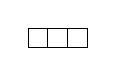
\begin{tikzpicture}[scale=0.25]
\draw(0,0)--(1,0)--(1,1)--(0,1)--cycle;
\draw(1,0)--(2,0)--(2,1)--(1,1)--cycle;
\draw(2,0)--(3,0)--(3,1)--(2,1)--cycle;\end{tikzpicture} or 
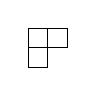
\begin{tikzpicture}[scale=0.25]
\draw(0,0)--(1,0)--(1,1)--(0,1)--cycle;
\draw(1,0)--(2,0)--(2,1)--(1,1)--cycle;
\draw(0,0)--(1,0)--(1,-1)--(0,-1)--cycle;\end{tikzpicture} or
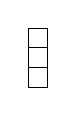
\begin{tikzpicture}[scale=0.25]
\draw(0,0)--(1,0)--(1,1)--(0,1)--cycle;
\draw(0,-1)--(1,-1)--(1,0)--(0,0)--cycle;
\draw(0,-2)--(1,-2)--(1,-1)--(0,-1)--cycle;\end{tikzpicture} .  There are several kinds of symmetic polynomials, \textbf{elementary symmetric polynomials}  and \textbf{complete symmetric polynomials} and \textbf{power sum symmetric polynomials}.  Our Galois Theory example seems to give the elementary symmetric polynomials.
$$ s({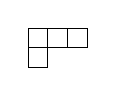
\begin{tikzpicture}[scale=0.25] 
\draw(0,0)--(1,0)--(1,1)--(0,1)--cycle;
\draw(1,0)--(2,0)--(2,1)--(1,1)--cycle;
\draw(2,0)--(3,0)--(3,1)--(2,1)--cycle;
\draw(0,0)--(1,0)--(1,-1)--(0,-1)--cycle;\end{tikzpicture}}) = s_{(2,1,1)} = \frac{1}{\Delta}
 \left| \begin{array}{ccc}   x_1^4 & x_2^4 & x_3^4 \\ x_1^2 & x_2^2 & x_3^2 \\ x_1 & x_2 & x_3 \end{array} \right| =  x_1 x_2 x_3(x_1 + x_2 + x_3) $$
\textbf{?} Do prime numbers over $\mathbb{Z}$ such as $5$ or $23$ factor in $\mathbb{Q}[x]/(x^3 - x - 1)$.  Find explicit factorizations.
\vfill
\begin{thebibliography}{} 

\item Henri Cohen \textbf{Computational Number Theory in Relation with L-Functions} \texttt{arXiv:1809.10904}

\end{thebibliography}

\end{document}